\RequirePackage[]{silence}
\WarningFilter{latex}{Marginpar on page}
\WarningFilter{lcg}{Using an already existing counter rand}
\documentclass[article, oneside]{aaltoseries}
\usepackage[utf8]{inputenc}
\usepackage[english]{babel}
\usepackage{IEEEtrantools}
\usepackage[hyphens]{url} % allow hyphens to break urls
\Urlmuskip=0mu  plus 1mu % allow for some spacing inside urls
\usepackage[hidelinks]{hyperref}
\usepackage[acronym]{glossaries}
\usepackage{amsfonts}
\usepackage{todonotes}
\usepackage[normalem]{ulem}
\usepackage{xcolor}
\usepackage{xspace}
\usepackage{textcomp}
\usepackage{etoolbox}
\usepackage[numbers]{natbib}
\newcommand{\TODO}[1]{\todo[inline]{#1}}
\newcommand{\jwnote}[1]{\todo[size=\small,color=blue!40]{#1}}
\newcommand{\JWNOTE}[1]{\todo[size=\small,inline,color=blue!40]{#1}}
\newcommand{\modif}[1]{\textcolor{blue}{#1}}
\newcommand\remove{\bgroup\markoverwith
{\textcolor{red}{\rule[0.5ex]{2pt}{0.8pt}}}\ULon}
\newcommand{\discuss}[1]{\todo[size=\small,color=green!40]{#1}}

\geometry{left=4cm,right=4cm,marginparwidth=3.5cm,marginparsep=5mm} % TODO: remove
% \geometry{left=1cm,right=7cm,marginparwidth=6.5cm,marginparsep=5mm} % TODO: remove
% \reversemarginpar % for todo notes on the wider side
\geometry{marginparwidth=5cm,marginparsep=3mm} % TODO: remove

% Use “\tocite{}” to get “citation needed” in document
\newcommand\tocite[1]{
	\todo{\ifstrempty{#1}{Citation needed}{#1}}
	[\,\textbf{\color{red}!}\,]
}


% ************************ Custom Referencing **********************************
\newcommand{\Fref}[1]{Figure~\ref{#1}}
\newcommand{\fref}[1]{figure~\ref{#1}}
\newcommand{\Tref}[1]{Table~\ref{#1}}
\newcommand{\tref}[1]{table~\ref{#1}}
\newcommand{\Eref}[1]{Equation~\ref{#1}}
\newcommand{\eref}[1]{equation~\ref{#1}}
\newcommand{\Sref}[1]{Section~\ref{#1}}
\newcommand{\sref}[1]{section~\ref{#1}}
\newcommand{\Lref}[1]{Listing~\ref{#1}}
\newcommand{\lref}[1]{listing~\ref{#1}}


\newcommand{\app}[1]{A\textsc{pp}$_{#1}$\xspace}

\newacronym{os}{OS}{operating system}
\newacronym{aosp}{AOSP}{Android Open Source Project}
\newacronym{vm}{VM}{virtual machine}

\title{Android App Collusion}


\author{Ervin Oro% Your first and last name: do _not_ add your student number
\\\textnormal{\texttt{ervin.oro@aalto.fi}}} % Your Aalto e-mail address
\affiliation{\textbf{Tutor}: Jorden Whitefield} % First and last name of your tutor

%==========================================================

\begin{document}
\bstctlcite{BSTcontrol}

\maketitle
\todo{set proper margins and document format}
%==========================================================

\begin{abstract}
\TODO{abstract}

\vspace{3mm}
\noindent KEYWORDS: \todo[inline, inlinewidth=5cm, noinlinepar]{list, of, key, words}

\end{abstract}

%============================================================

\section{Introduction}
\label{sec:intro}

Android is an \gls{os} that is primarily designed for mobile devices, e.g., smartphones and tablets. With more than two billion active devices~\cite{AOSP2018}, it is estimated to be the most widely used \gls{os}, surpassing even Microsoft Windows~\cite{AWSLLC2018, StatCounter2018}. Android is designed to be an open platform: developed and maintained by Google LLC, but largely released as the \gls{aosp} for everyone to study and evaluate \cite{AOSP}. The Android \gls{os} includes support for apps, which are easily installable application packages that can extend the functionality of devices. Apps can be developed and distributed by anyone with very low barrier of entry.

While this popularity of Android is not reflected by the proportion of malware attacks, most of which still target Windows, both the number and complexity of attacks against Android are increasing~\cite{AVTESTGH2018}\todo{graph from this source could be added}. This is especially troublesome as many people increasingly rely on their smartphones -- often to store their personal data, online account credentials, money, and more. \citeauthor{McAfee2018} estimates that revenues for mobile malware authors could be in the billion-dollar range by 2020 \cite{McAfee2018}.

Given the increasing potential damage from Android malware, defending against it is an active area of research. Android uses a \todo{figure depicting multi-layer security could be added}multi-layer security approach, combining machine learning, platform security and secure hardware~\cite{AOSP2018}. Machine learning methods are utilised by Google Play Store to prevent uploading potentially harmful applications, and by Google Play Protect~\cite{AOSPplayprotect} to scan apps locally on users' devices. Android's platform security has been enhanced over the years with the addition of multiple security features, for example, SELinux protections~\cite[\href{https://source.android.com/security/selinux}{``Security-Enhanced Linux in Android''}]{AOSPsecurity}, exploit mitigations~\cite{Edge2016}, privilege reductions~\cite{Lawrence2017}, and encryption. Recent versions of Android leverage hardware security features, including keystore and remote key attestation~\cite{Willden2017}, and receive regular software updates. These security mechanisms have been partially successful, as exploit pricing and difficulty are growing by some estimates~\cite{AOSP2018}.

However, malicious actors are continuously developing exploits to bypass existing protections, and a number of threats, e.g., app collusion, cannot yet be reliably detected nor defended against. App collusion is a secret collaboration between apps with malicious intentions (\Sref{sec:def}). This can be facilitated by any of the numerous ways for apps to communicate with each other that the Android system provides (\Sref{sec:methods}). Methods for apps to collude also exist on the iOS platform \cite{Deshotels2016}. Given a malicious app that would be detected and blocked with state of the art security systems, its functionality can be split into several apps, so that each of them would be categorised as benign when analysed separately~\cite{Chen2018}.

Android app collusion is not a new concept~\cite{Schlegel2011}, and multiple attempts have been made to develop suitable detection systems (\Sref{sec:approaches}). Computationally simple but very coarse filters have been developed based on statically extracted features of apps \cite{Asavoae2016, Chen2018}, while computationally expensive and more accurate filters have used formal modelling of Android apps \cite{Asavoae2018} or modified versions of the Android \gls{os} \cite{Enck2014} to track information flows. Heuristic approaches and manual analysis has also been proposed \cite{Muttik2016}.

Despite this, there are currently no robust and usable ways to detect app collusions. Existing solutions have large number of false negatives, false positives, or they are infeasibly difficult to implement. The number of possible combinations of $N$ apps is $N^N$, and Google Play Store alone is reported to host more than 2.6 million apps~\cite{Statista2018}. Most proposed solutions therefore apply very aggressive filtering, causing only some malicious combinations to be included into analysis, and others to be reported as false negatives. Furthermore, most proposed solutions have a large number of false positives due to their inability to differentiate collusion from legitimate collaboration. Some have experimented with checking apps manually to determine their intentions~\cite{Muttik2016}, but this demands even more aggressive filtering. Therefore, app collusion remains an open research challenge.

Furthermore, existing literature on the topic has significant limitations. Some influential work in the field is now outdated and has not been updated. Many authors have defined app collusion for themselves in ways that are simpler to detect but not applicable in the real world, often including large amounts of legitimate apps. Some published information also has credibility issues, either dismissing prior work by claiming that collusion is a new idea, or claiming that they have solved the problem without providing sufficient evidence.

This report aims to provide an overview of app collusion on the Android platform as follows. \Sref{sec:def} discusses the nature and definitions of app collusion,~\Sref{sec:methods} provides specific overview of methods that can be used for colluding on Android,~\Sref{sec:examples} describes known examples of colluding apps, and~\Sref{sec:approaches} gives an overview of approaches that have been taken to collusion detection and their limitations.

\section{Description and definition of app collusion}
\label{sec:def}

The Oxford English Dictionary defines collusion as ``Secret agreement or understanding for purposes of trickery or fraud; underhand scheming or working with another; deceit, fraud, trickery''~\cite{OEDcollusion}. \citeauthor{Asavoae2017}~\cite{Asavoae2017} define collusion for the case of Android apps as the situation where several apps are working together in performing a threat. According to these definitions, app collusion must have the following three properties:

\begin{enumerate}
	
	\item Colluding apps must be working together secretly. Conversely, apps working together in collaboration is common and encouraged practice when such collaboration is well documented \cite[\href{https://developer.android.com/training/basics/intents}{``Interacting with Other Apps''}]{AOSPdeveloper}.

	\item All colluding apps must be in agreement. A distinctly different but related concept is the ``confused deputy'' attack, where one app mistakenly exposes itself to other installed apps \tocite{Hardy, N.: The confused deputy:(or why capabilities might have been invented. ACMSIGOPS Operating Systems Review 22(4), 36–38 (1988)}.

	\item Colluding apps must have malicious intentions. The intentions of Android app collusion would then be to violate one of Android's security goals, which are defined in \cite{AOSPsecurity} as:
	\begin{singleenums}
		\item to protect app data, user data, and system resources (including the network),
		\item to provide app isolation from the system, other apps, and the user.
	\end{singleenums}
\end{enumerate}
\\\todo{formatting}
It is important to note that the goal 3(b) is not to enforce isolation, but to provide isolation for those who require it. As such, apps working together do not automatically violate goal 3(b), but it would be collusion if apps worked together to break isolation with some other non-content app, the system, or the user.

\TODO{many things affect, including non technical}

\TODO{difficult to distinguish}

\TODO{alternative definition \cite{Xu2017}}

\section{Methods for colluding}
\label{sec:methods}

By default, all Android apps run in separate sandboxes~\cite[\href{https://source.android.com/security/overview/app-security}{``Application security''}]{AOSPsecurity}, which are based on user separation by the Linux kernel, and enhanced by SELinux and \texttt{seccomp}~\cite[\href{https://source.android.com/security/app-sandbox}{``Application Sandbox''}]{AOSPsecurity}. By default, all communication between these sandboxes is blocked, but apps can open certain communication channels or prevent being separated into different sandboxes altogether. Some channels, so-called overt channels, are designed to be used by apps to communicate, while others, so-called covert channels, utilise functionalities which were originally intended for other purposes. All channels discussed below require the participation of both parties, but some researchers have looked into ways to cross sandbox borders unilaterally, therefore breaking the goal 3(b) in \sref{sec:def}~\tocite{}.

\subsection{Overt channels}
\label{sec:overt}

The \citeauthor{AOSPsecurity}~\cite{AOSPsecurity} describes channels designed for inter-app communication, such as sandbox sharing and binder, on pages \href{https://source.android.com/security/overview/app-security}{``Application security''} and \href{https://source.android.com/security/app-sandbox}{``Application Sandbox''}.

Apps published by the same entity may share a sandbox. In this case, there are no restrictions for their communication. These apps can use any of the traditional UNIX-type mechanisms, including filesystem, local sockets, or signals.

When apps are running in different sandboxes, the Linux kernel prevents these sandboxed apps from accessing each other's processes or files. In older Android versions, only Linux discretionary access control was used, allowing apps to make their files world-accessible, but newer versions of Android forbid this using SELinux mandatory access control rules. Many works\tocite{} discuss the use of shared preferences to exchange information between apps, but since shared preferences relied internally on files being world-accessible, this approach is no longer viable. Apps can still use any file-based communication methods when they have permission to access the external storage, but this way users would know that such communication may take place.

However, Android also provides a method for apps to communicate without any user-granted permission or visibility. This is enabled by a remote procedure call mechanism called binder\todo{revisit after \sref{sec:approaches}: if it discusses more about binder; it needs to be introduces more - a short introduction to Android platform architecture with figure. See \url{https://developer.android.com/guide/platform}}. Any app can send messages to the binder arbitrarily, but other apps must explicitly start listening and accept incoming communications. The Android platform provides three main ways to do this:
\begin{enumerate}
	\item Services~\cite[\href{https://developer.android.com/guide/components/services}{``Services overview''}]{AOSPdeveloper}: Apps may start services, which can provide interfaces that are directly accessible using binder.
	\item Intent filters~\cite[\href{https://developer.android.com/guide/components/intents-filters}{``Intents and Intent Filters''}]{AOSPdeveloper}: Intents are simple message objects that represents an intention to do something. Apps may ask some part of them to be executed when an intent with certain properties matching their filter is initiated.
	\item ContentProviders~\cite[\href{https://developer.android.com/guide/topics/providers/content-providers}{``Content providers''}]{AOSPdeveloper}: Apps can define ContentProviders to expose some of their data.
\end{enumerate}
\TODO{Maybe add something about android platform architecture. Figure 1. Explicit/implicit intents.}

The binder provides an easy way for apps to communicate with each other, promoting openness and allowing a separation of concerns. Examples include apps using an intent to ask the camera app to take a photo instead of asking camera control permission, and communication apps allowing other apps to share data through itself. Binder has a well-defined interface that could be monitored.

\subsection{Covert channels}
\label{sec:covert}

In addition to the overt channels, a large amount of covert channels have been discovered. \citeauthor{Marforio2012}~\cite{Marforio2012} propose a classification of communication channels based on whether Application level APIs, \Gls{os} native calls, or Hardware functionalities are utilised. \citeauthor{Al-Haiqi2014}~\cite{Al-Haiqi2014} describe categorising covert channels as either timing or storage channels. However, neither of these categorising approaches provide clear boundaries in all cases nor cover all possible covert channels, which by their nature form an unbounded set. This section provides some examples of covert channels in Android.

\citeauthor{Schlegel2011}~\cite{Schlegel2011} show that any application can change the vibrate setting and use intent filters to be notified every time the setting is changed without requiring specific permissions, therefore demonstrating that apps can create an information channel using the vibrate setting.  Similarly, the volume setting can be used. While apps cannot subscribe to be notified when volume is changed and have to manually check this setting, it has the benefit of having 8 different states, as opposed to the vibrate setting, which is a boolean value. These channels are invisible to users, as long as data transmission does not coincide with audio playback or receiving notifications.

\citeauthor{Marforio2012}~\cite{Marforio2012} describe how data could be exchanged between colluding apps by modifying and monitoring the number of threads, processor usage, and free space on filesystem. However, the APIs they used have since been deprecated \cite{nn2017}. Nevertheless, scanning the current Android documentation with their ideas in mind yields some results that might allow similar attacks to be mounted on recent versions of Android. For example, free disk space can be queried through the \href{https://developer.android.com/reference/android/os/StatFs.html#getAvailableBlocksLong()}{StatFs\#getAvailableBlocksLong()} API on latest Android versions \cite{AOSPdeveloper}. However, a proof of concept should be created before this method can be assumed to be viable.

The system load can also be measured indirectly to transmit information \cite{Marforio2012}. In this scenario, the transmitting app modulates data payload by varying the load on the system. The receiving app then repeatedly runs a CPU-intensive computation and measures the time it takes to complete, in order to infer whether or not the transmitting app is loading the system or not. This approach was shown to work even when receiver is just some JavaScript in the browser and not an installed Android app.

Another approach is presented by \citeauthor{Al-Haiqi2014}~\cite{Al-Haiqi2014}, where one app utilises the vibration motor to transmit data, and another app uses the accelerometer readings to receive that data. This is further developed by \citeauthor{Qi2018}~\cite{Qi2018}, who propose covert channels based on user behaviour. Instead of using the vibration motor, a transmitting app could prompt the user to move their phone in certain ways, for example, posing as a rally game where the user needs to turn their phone at specific times based on a track generated by the malicious app.
\\
\TODO{Add a subsection conclusion paragraph}

\section{Examples of Android app collusion}
\label{sec:examples}

A basic example of app collusion (\Fref{fig:sample}) is as follows:
\begin{singleenums}
	\item \app{A} obtains some private information.
	\item \app{A} transmits the information to \app{B} using some overt or covert channel.
	\item \app{B} exfiltrates the information over the internet.
\end{singleenums}

\begin{figure}[h]
	\centering
	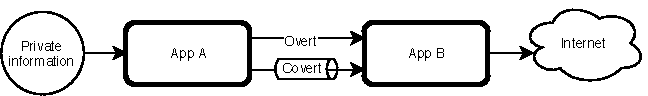
\includegraphics[width=1.0\textwidth]{figures/Collusion1}
	\caption{Structure of a basic app collusion example.}
	\label{fig:sample}
\end{figure}

An early example of this kind of collusion was described by \citeauthor{Schlegel2011}~\cite{Schlegel2011}. In their case, \app{A} was the Soundcomber app that obtained private information using the microphone. To avoid detection, the Soundcomber app did not have permission to access the internet, so they proposed to use a second app to exfiltrate the information. Similar hypothetical example is also described by \citeauthor{Asavoae2017}~\cite{Asavoae2017}, where \app{A} would be a contacts app with READ\_CONTACTS permission, and \app{B} would be a weather app with INTERNET permission. However, no such examples have been reported in the wild.

There is one known example of app collusion in the wild reported by \citeauthor{Blasco2016}~\cite{Blasco2016}. They noticed a set of apps from different vendors by manual review of apps that were previously labelled as potentially unwanted, and were capable of accessing shared preferences files from different apps. All of these apps included a library, known as MoPlus SDK, that was known to contain remote-control capability.

\TODO{Add figure depicting the MoPlus SDK}

The MoPlus SDK may be embedded into many different apps, with 20 such being identified by \cite{Blasco2016}. It can then open a local HTTP server allowing the attacker to abuse any permissions given to its host app. With potentially many instances of the MoPlus SDK running on the same device with different permissions, they would work together to guarantee that only the instance with highest level of permissions is the one that starts accepting remote commands. No sensitive information is exchanged between the apps, but still all three properties of app collusion are present.

\section{Existing methods for detecting collusions}
\label{sec:approaches}

Attempts with various scopes and outcomes have been made to detect app collusion. Results range from relatively computationally easy but very coarse filters to more accurate but very expensive approaches.

\subsection{Based on permissions/interfaces}
\label{sec:filter}

The simplest approach is to base the analysis on statically extracted features of apps, such as the set of permissions declared in their manifests or the set of Android APIs they import. This way large amounts of apps can be quickly scanned, but necessarily only rough estimations can be made, since very little information about the app is actually used in decision making.

For example, \citeauthor{Asavoae2016}~\cite{Asavoae2016} describe a filtering method based on app's API calls and the permissions declared in its manifest file. They define collusion as a pair of apps that satisfy these three conditions:
\begin{enumerate}
	\item First app declares a permission that they classified as giving access to sensitive information.
	\item Second app declares a permission that they classified as giving app the ability to send information to the outside world.
	\item Finally, first app must be able to send, and second app able to receive on the same channel. They consider the following channels:
	\begin{singleitems}
		\item Intents (each action separately)
		\item External storage
	\end{singleitems}
	(They also consider shared preferences, each file separately, but this is now deprecated: \Sref{sec:overt})
\end{enumerate}
It is not clear from their description, but can be assumed, that they further ignore apps that match both first and second criteria, because otherwise their filter would simply detect any app pairs that can communicate using one of these channels. They claim that this approach over-approximates the set of colluding apps, while actually it must be noted that they only consider a narrow subset of app collusions, and, for example, the MoPlus SDK would be labelled as benign by this approach.

\citeauthor{Chen2018}~\cite{Chen2018} propose a similar approach. First, they notice that exists a machine learning algorithm that, given the set of all API calls in an app, can predict whether the app is malicious or not. For communication they only consider intents as a possible channel. For each app they detect which intents it can send and receive, and then they group together apps that could communicate with each other. Finally, to detect, whether a group of apps is benign or malicious, they pass the union of all API calls of the apps in the group to the aforementioned machine learning algorithm.

Neither of these approaches can detect if apps actually communicate with each other, nor what kind of information is exchanged between apps if they do communicate, since they use no information about the order of operations within apps. They both consider only limited overt channels.

\subsection{Based on control flow analysis}
\label{sec:flow}

A more accurate detection of collusion can be achieved when the code of apps is also analysed to detect whether or not they communicate, and what kind of information can they exchange. Model-based and runtime approaches have been taken to that.

\citeauthor{Asavoae2018}~\cite{Asavoae2018} describe a method checking, whether information theft through collusion exists within the set of possible control flows for an app. They propose annotating each object with current app ID and boolean ``sensitive'' when it is returned by one of predefined Android APIs. Whenever an object is used, its sensitivity and app ID values are propagated to all resulting objects. Input set of apps is considered to be colluding if an object marked sensitive is passed to one of predefined exporting Android APIs so that the current app ID is different to the app ID from the object. They explore analysing concrete semantics, in which case the analysis takes longer, or even forever when the app code contains any loops, and propose a abstraction of Android app semantics, which is less accurate, but guaranteed to provide an answer. They only consider intent based inter-app communication.

Another approach is to modify the Android \gls{os} to track information flow at runtime. Example of this is TaintDroid \cite{Enck2014}, which can track information flows from sensitive sources to sensitive sinks system wide, but incurs $14\%$ CPU overhead doing so. They use variable-level label tracking within app code (by augmenting the Java \gls{vm}), message-level tracking in Binder, method-level tracking for native system libraries, and file-level tracking. Therefore, this approach is only capable of tracking information flow within Java code, intents, Android API calls, and files, but native code is not tracked (authors here approached this by banning all native components in apps, breaking $5\%$ of apps by some estimates). Use of labels is similar to \cite{Asavoae2018}, but amount of false positives is much smaller, because corresponding exit state must be actually reached for it to be reported. False negatives may be caused when labels are not propagated through covert channels, and false positives when label propagation is overly conservative.

\subsection{Other}
\label{sec:othermethods}

None of the above approaches have been able to detect collusion using covert channels. People have looked into closing some covert channels, but it is not reasonable to assume that all covert channels can be found. Additionally, even today there exist known open covert channels.

\citeauthor{Muttik2016}~\cite{Muttik2016} proposes augmenting aforementioned approaches with additional heuristic rules. He argues that colluding apps can be also detected by indirect signals, for example whether apps come from the same source, explicitly encourage co-installation, are frequently installed together, use similar libraries, etc. Furthermore, he notes that signals like publication date, app market and installation method can be used. Finally, \citeauthor{McAfee2016} also claims to use manual review and reverse engineering to make final decisions about apps.

Already in 2016 \citeauthor{McAfee2016} claimed that their product is able to detect colluding mobile apps and stop them from running \cite{McAfee2016}. However, based on known information about the state of the art, this is unlikely to be entirely true.

\section{Conclusion}
\label{sec:conclusion}

%============================================================

\bibliographystyle{IEEEtranN}
\bibliography{ieee,oro-cs-seminar}
\TODO{format bibliography - remove urls from non-online sources}

\listoftodos
\TODO{remove list of todos}

\end{document}
